\begin{frame}
    \frametitle{Научная новизна}
    \begin{itemize}

    \item В настоящей работе максимизируется излучение в одном заданном направлении, что в наибольшей степени соответствует системам коротковолновой радиосвязи.
    \item Разработаны реализации алгоритмов с процедурой возвращения в допустимую область.
    \item Обоснован подход к снижению размерности задачи фиксированием значения переменной.
    \item Впервые показано наличие кластеров из локальных оптимумов.
    \item На открытый вопрос о целесообразности учета взаимного влияния излучателей при оптимизации направленности ФАР КВ диапазона дан положительный ответ.
    \item Впервые показана нецелесообразность использования широкополосных вертикальных излучателей в составе ФАР коротковолнового диапазона.
    \end{itemize}
\end{frame}
\note{
    Проговаривается вслух научная новизна
}

\begin{frame}
    \frametitle{Научная и практическая значимость}
    \begin{itemize}
        \item Разработанные алгоритмы оптимизации возбуждения ФАР могут  применяться в системах связи коротковолнового диапазона для увеличения дальности, снижения энергозатрат или площади, занимаемой антеннами. Созданное программное обеспечение позволяет производить необходимые для этого расчеты.
        \item Полученное обоснование необходимости учета взаимного влияния излучателей при оптимизации напраленности ФАР, а также результаты вычислительных экспериментов для различных вариантов ФАР могут быть полезны при проектировании новых антенных систем.

    \end{itemize}
\end{frame}
\note{
    Проговариваются вслух научная и практическая значимость
}

%\begin{frame}
%    \frametitle{Свидетельство о регистрации программы}
%    \begin{figure}[h]
%        \centering
%        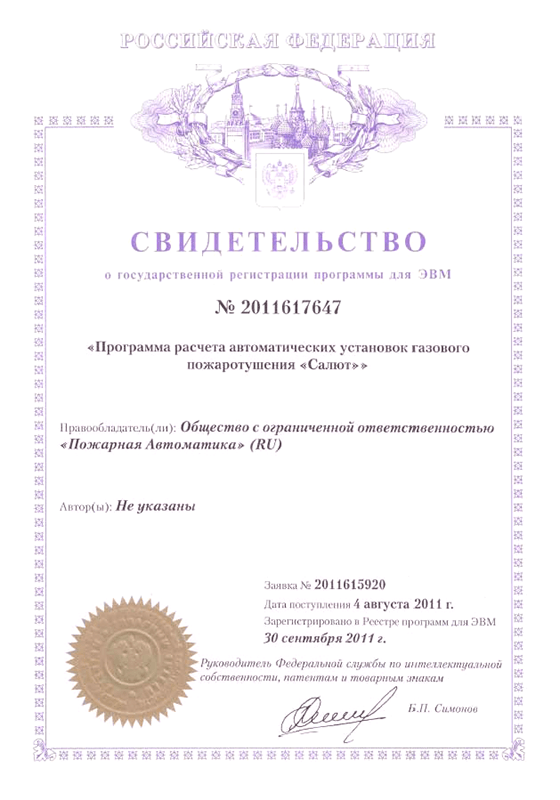
\includegraphics[height=0.7\textheight]{registration}
%    \end{figure}
%\end{frame}
%\note{
%    Получено свидетельство о регистрации разработанной программы \textsc{Hello~world™}.
%}

%\begin{frame}
%    \frametitle{Акт о внедрении}
%    \begin{figure}[h]
%        \centering
%        \fbox{
%            \begin{minipage}[t]{0.4\linewidth}
%                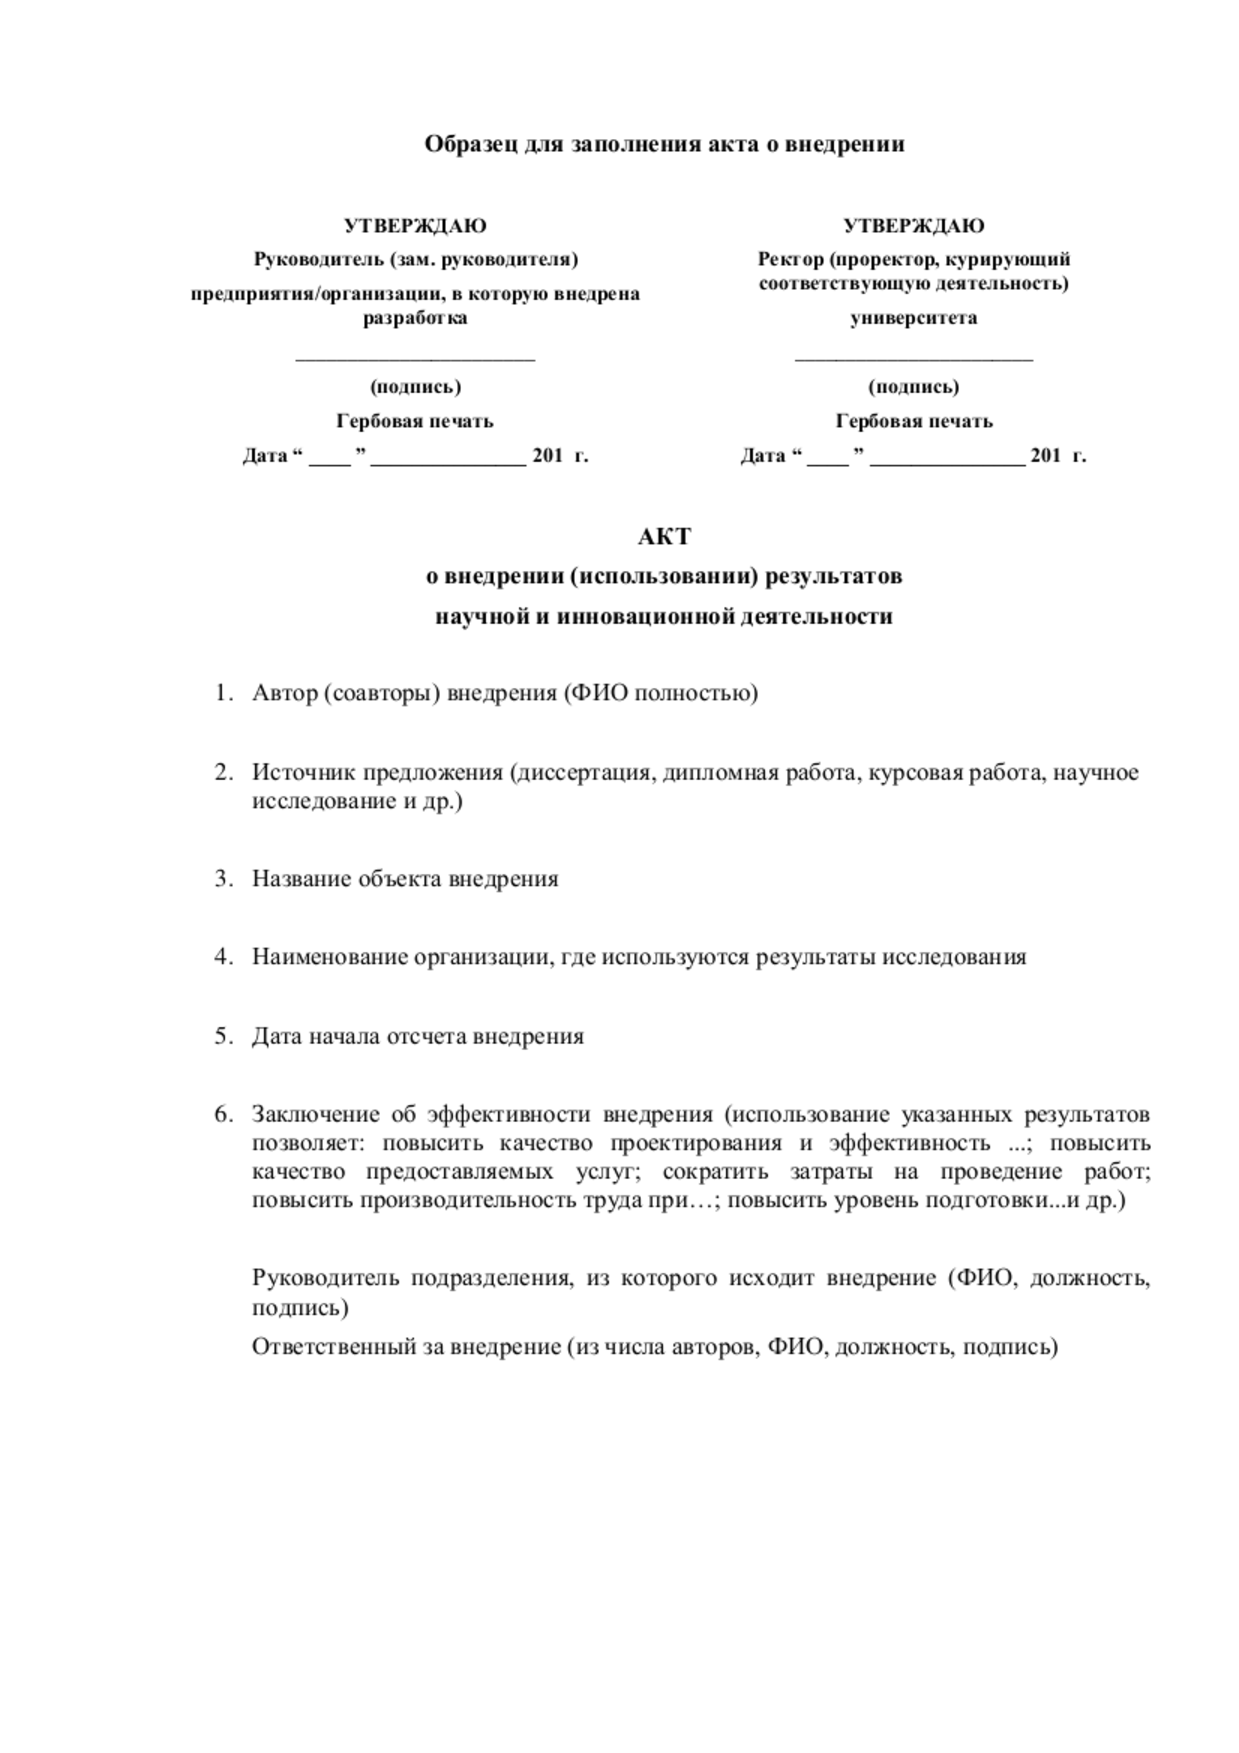
\includegraphics[width=\linewidth]{implementation}
%            \end{minipage}
%        }
%    \end{figure}
%\end{frame}
%\note{
%    Получен акт о внедрении.
%}

%\begin{frame} % публикации на одной странице
 \begin{frame}[t,allowframebreaks] % публикации на нескольких страницах
    \frametitle{Основные публикации}
    \nocite{tyu:daor}%
    \nocite{tyu22:reis}%
    \nocite{tyu:jphys}%
    \nocite{tyu:fmh}%
    \nocite{tyu:reis}%
    \nocite{tyu:opta}%
    \nocite{tyu:motor}%
    \ifnumequal{\value{bibliosel}}{0}{
        \insertbiblioauthor
    }{
        \printbibliography%
    }
\end{frame}
\note{
    Результаты работы опубликованы в N печатных изданиях,
    в~т.\:ч. M реферируемых изданиях.
}

\begin{frame}
    \frametitle{Участие в конференциях}
    \begin{itemize}
      \item VII Международной конференции «Проблемы оптимизации и их приложения» - Омск, июль 2018.
      \item Международной конференции «Теория математической оптимизации и исследование операций» - Екатеринбург, июль 2019.
      \item V Международной научно-технической конференции «Радиотехника, электроника и связь» - Омск, октябрь 2019.
      \item Международнаой конференции «Теория математической оптимизации и исследование операций» - Иркутск, июль 2021.
    \end{itemize}
\end{frame}
\note{
    Работа была представлена на ряде конференций.
}

\begin{frame}[plain, noframenumbering] % последний слайд без оформления
    \begin{center}
        \Huge
        Спасибо за внимание!
    \end{center}
\end{frame}
